 % mainfile: ../../../../master.tex
\label{task:20240409_aosp}


\subsection{Recompile AOSP 13}

\subsubsection{Why is it not logging to Logcat?}

Log is not showing, even if \path{LOG_NDEBUG} is set to \texttt{0} in \texttt{AndroidRuntime.cpp}.

Okay, now it works and I didn't edit anything further.

\subsection{Which components are involved in ART?}
Finishing up the sequence flow.

\subsection{Components of Debloater Flow in AOSP 13} 

\subsubsection{ART Procedures in Debloating Flow}

\begin{longtable}{p{.350\linewidth}p{.65\linewidth}} 
\toprule
File & Procedure  \\
\midrule
\endhead

\path{libartbase} \\

\path{os_linux.h}
&Add declaration \path{CreateMINIMAFile}
\\

\path{os_linux.h}
&Add declaration \path{CreateDirectories2}
\\

\path{os_linux.cc}
&Add definition \path{CreateMINIMAFile}
\\

\path{os_linux.cc}
&Add definition \path{CreateDirectories2}
\\

\midrule
\path{libdexfile} \\

\path{art_dex_file_loader.cc}
&Modify definition \path{ArtDexFileLoader::Open}
\\

\path{dex_file_loader.cc}
&Modify definition \path{DexFileLoader::OpenCommon}
\\

\midrule
\path{libnativeloader} \\

\path{native_loader_namespace.cpp}
&Modify definition \path{NativeLoaderNamespace::Load}
\\

\path{native_loader.cpp}
&Modify definition \path{OpenNativeLibrary}
\\

\path{native_loader.cpp}
&Modify definition \path{OpenNativeLibraryInNamespace}
\\

\midrule
\path{oderefresh} \\

\path{oderefresh.cc}
&Modify definition \path{AddDex2OatProfileAndCompilerFilter}
\\

\path{oderefresh_main.cc}
&Modify definition \path{InitializeConfig}
\\

\midrule
\path{runtime} \\

\path{app_info.h}
&Add declaration \path{GetPackageName}
\\

\path{app_info.cc}
&Modify definition \path{GetPackageName}
\\

\path{art_method-inl.h}
&Modify declaration \\
& \path{ArtMethod::CheckIncompatibleClassChange} \\

\path{art_method-inl.h}
&Modify declaration \\
& \path{ArtMethod::UpdateCounter} \\


\path{art_method.h}
&Modify declaration  \path{ArtMethod::UpdateCounter}
\\

\path{art_method.cc}
&Modify declaration \path{ArtMethod::Invoke}
\\

\path{art_method.cc}
&Modify declaration \path{ArtMethod::PrettyMethod}
\\

\path{class_linker.cc}
&Modify declaration \path{ClassLinker::FindClass}
\\

\path{class_linker.cc}
&Modify declaration \path{LinkCode}
\\

\path{class_linker.cc}
&Modify declaration \path{ClassLinker::LoadClass}
\\

\path{instrumentation.cc}
&Modify declaration \path{CanUseNterp}
\\

\path{instrumentation.cc}
&Modify declaration \path{Instrumentation::InitializeMethodsCode}
\\

\path{oat_file_manager.cc}
&Modify declaration \path{OatFileManager::OpenDexFilesFromOat_Impl}
\\

\path{runtime.h}
&Add declaration \path{struct} \path{NativeLibFunc;}
\\

\path{runtime.h}
&Add declaration \path{MYmatch_hook_method}
\\

\path{runtime.h}
&Add declaration \path{MYmatch_target_method}
\\

\path{runtime.h}
&Add declaration \path{MYreadFile}
\\

\path{runtime.h}
&Add declaration \path{MYmake_file}
\\

\path{runtime.h}
&Add declaration \path{read_content}
\\

\path{runtime.h}
&Add definition \path{getLoadingSchema}
\\

\path{runtime.h}
&Add definition \path{getLoadedSchema}
\\

\path{runtime.h}
&Add definition \path{getShouldReadSchema}
\\

\path{runtime.h}
&Add definition \path{setLoadingSchema}
\\

\path{runtime.h}
&Add definition \path{setLoadedSchema}
\\

\path{runtime.h}
&Add definition \path{setShouldReadSchema}
\\

\path{runtime.h}
&Add definition \path{getDebugging}
\\

\path{runtime.h}
&Add definition \path{getTarget_method_string_vector}
\\

\path{runtime.h}
&Add definition \path{setTarget_method_string_vector}
\\

\path{runtime.h}
&Add definition \path{getMINIMA_file_path}
\\

\path{runtime.h}
&Add definition \path{getMINIMA_folder_path}
\\

\path{runtime.h}
&Add definition \path{getHookMethodName}
\\

\path{runtime.h}
&Add declaration \path{MINIMA_file_path}
\\

\path{runtime.h}
&Add declaration \path{hook_method_name}
\\

\path{runtime.h}
&Add declaration \path{target_method_string_vector}
\\

\path{runtime.h}
&Add declaration \path{target_native_func_string_vector}
\\

\path{runtime.h}
&Add declaration \path{debugging}
\\

\path{runtime.h}
&Add declaration \path{api_prefix_List}
\\

\path{runtime.h}
&Add declaration \path{loaded_schema_}
\\

\path{runtime.h}
&Add declaration \path{loading_schema_}
\\

\path{runtime.h}
&Add declaration \path{should_read_schema_}
\\

\path{runtime.cc}
&Add definition \path{StringAppendV}
\\

\path{runtime.cc}
&Add definition \path{StringPrintf}
\\

\path{runtime.cc}
&Add definition \path{StringAppendF}
\\

\path{runtime.cc}
&Add definition \path{Runtime::MINIMA_file_path}
\\

\path{runtime.cc}
&Add definition \path{Runtime::hook_method_name}
\\

\path{runtime.cc}
&Add definition \path{Runtime::debugging}
\\

\path{runtime.cc}
&Add definition \\
&\path{Runtime::target_method_string_vector}
\\

\path{runtime.cc}
&Add definition \\
&\path{Runtime::target_native_func_string_vector}
\\

\path{runtime.cc}
&Add definition \path{api_prefix_List}
\\

\path{runtime.cc}
&Add definition \path{NativeLibFunc}
\\

\path{runtime.cc}
&Modify definition \path{Runtime}
\\

\path{runtime.cc}
&Modify definition \path{Create}
\\

\path{runtime.cc}
&Modify definition \path{Start}
\\

\path{runtime.cc}
&Modify definition \path{Init}
\\

\path{runtime.cc}
&Add definition \path{MYmatch_hook_method}
\\

\path{runtime.cc}
&Add definition \path{java2cpp}
\\

\path{runtime.cc}
&Add definition \path{is_within_JNImethod_list}
\\

\path{runtime.cc}
&Add definition \path{Runtime::read_content}
\\

\path{runtime.cc}
&Add definition \path{is_packageMethod}
\\

\path{runtime.cc}
&Add definition \path{Runtime::MYmatch_target_method}
\\

\path{runtime.cc}
&Add definition \path{Runtime::MYmake_file}
\\

\path{runtime.cc}
&Add definition \path{Runtime::MYreadFile}
\\

\path{trace.cc}
&Add definition \path{modifyFilePermissions}
\\

\path{trace.cc}
&Modify definition \path{Trace::Start}
\\

\path{trace.cc}
&Modify definition \path{Trace::Trace}
\\

\path{trace.cc}
&Modify definition \path{Trace::MethodEntered}
\\

\path{trace.cc}
&Modify definition \path{Trace::MethodExited}
\\

\midrule
\path{runtime/entrypoints} \\

\path{quick_trampoline_entry_points.cc}
&Modify definition \path{artQuickToInterpreterBridge}
\\

\midrule
\path{runtime/interpreter} \\

\path{interpreter_common.cc}
&Modify definition \path{DoCallCommon}
\\

\path{interpreter_switch_impl-inl.h}
&Modify definition \path{ExecuteSwitchImplCpp}
\\

\path{interpreter_switch_impl.h}
&Modify definition \path{ExecuteSwitchImpl}
\\

\path{interpreter.cc}
&Modify definition \path{Execute}
\\

\path{interpreter.cc}
&Modify definition \path{EnterInterpreterFromEntryPoint}
\\

\midrule
\path{runtime/jit} \\

\path{jit.cc}
&Modify definition \path{MethodEntered}
\\

\midrule
\path{runtime/jni} \\

\path{java_vm_ext.cc}
&Modify definition \path{FindSymbol}
\\

\path{java_vm_ext.cc}
&Modify definition \path{JavaVMExt::LoadNativeLibrary}
\\

\path{jni_internal.cc}
&Modify definition \path{FindClass}
\\

\midrule
\path{runtime/mirror} \\

\path{class.cc}
&Modify definition \path{FindClassMethodWithSignature}
\\

\midrule
\path{runtime/native} \\

\path{dalvik_system_DexFile.cc}
&Modify definition \path{DexFile_openDexFileNative}
\\

\path{dalvik_system_ZygoteHooks.cc}
&Add definition \path{modifyFilePermissions1}
\\

\path{dalvik_system_ZygoteHooks.cc}
&Modify definition \path{ZygoteHooks_nativePostForkChild}
\\

\midrule
\caption{ART Procedures involved in Debloation} 
\label{tab:debloatartprocedures}
\end{longtable}

\subsubsection{Bionic Procedures in Debloating Flow}

\begin{longtable}{p{.50\linewidth}p{.50\linewidth}} 
\toprule
File & Procedure  \\
\midrule
\endhead

\path{libc} \\

\path{execinfo/include/bionic/execinfo.h}
&Delete evertyhing and add \\
&\path{../../../include/execinfo.h}
\\

\path{fts/include/bionic/fts.h}
&Delete evertyhing and add \\
&\path{../../../include/fts.h}
\\

\midrule
\path{libdl} \\

\path{libdl.cpp}
&Modify definition \path{android_dlopen_ext}
\\

\midrule
\path{linker} \\

\path{dlfcn.cpp}
&Modify definition \path{dlopen_ext}
\\

\path{dlfcn.cpp}
&Modify definition \\
&\path{__loader_android_dlopen_ext}
\\

\path{linker_phdr.h}
&Add declaration \path{add_de_lib_name_vec}
\\

\path{linker_phdr.h}
&Add declaration \path{add_de_func_name_vec}
\\

\path{linker_phdr.h}
&Add declaration \path{match_target_so_name}
\\

\path{linker_phdr.h}
&Add declaration \path{match_target_func_name}
\\

\path{linker_phdr.h}
&Add declaration \path{dynsym_fragment_}
\\

\path{linker_phdr.h}
&Add declaration \path{dynsym_table_}
\\

\path{linker_phdr.h}
&Add declaration \path{de_dynsym_vec}
\\

\path{linker_phdr.h}
&Add declaration \path{de_func_name_vec}
\\

\path{linker_phdr.h}
&Add declaration \path{de_natlib_name_vec}
\\

\path{linker_phdr.h}
&Add declaration \path{handled_array}
\\

\path{linker_phdr.cpp}
&Add definition \path{debug_zicheng_native}
\\

\path{linker_phdr.cpp}
&Modify definition \path{ElfReader}
\\

\path{linker_phdr.cpp}
&Modify definition \path{ElfReader::Load}
\\

\path{linker_phdr.cpp}
&Add definition \path{compareDynsymPointers}
\\

\path{linker_phdr.cpp}
&Add definition \path{compareDynsyms}
\\

\path{linker_phdr.cpp}
&Modify definition \\
&\path{ElfReader::ReadProgramHeaders}
\\

\path{linker_phdr.cpp}
&Modify definition \\
&\path{ElfReader::ReadSectionHeaders}
\\

\path{linker_phdr.cpp}
&Modify definition \\
&\path{ElfReader::ReadDynamicSection}
\\

\path{linker_phdr.cpp}
&Modify definition \\
&\path{phdr_table_get_load_size}
\\

\path{linker_phdr.cpp}
&Modify definition \\
&\path{ElfReader::ReserveAddressSpace}
\\

\path{linker_phdr.cpp}
&Modify definition \\
&\path{ElfReader::LoadSegments}
\\

\path{linker_phdr.cpp}
&Add definition \\
&\path{ElfReader::add_de_func_name_vec}
\\

\path{linker_phdr.cpp}
&Add definition \\
&\path{ElfReader::add_de_lib_name_vec}
\\

\path{linker_phdr.cpp}
&Add definition \\
&\path{ElfReader::match_target_so_name}
\\

\path{linker_phdr.cpp}
&Add definition \\
&\path{ElfReader::match_target_func_name}
\\

\path{linker.cpp}
&Modify definition \\
&\path{open_library_in_zipfile}
\\

\path{linker.cpp}
&Modify definition \path{find_libraries}
\\

\path{linker.cpp}
&Modify definition \path{find_library}
\\

\path{linker.cpp}
&Modify definition \path{do_dlopen}
\\

\midrule
\caption{Bionic Procedures involved in Debloation} 
\label{tab:debloatbionicprocedures}
\end{longtable}

\subsubsection{Framework Procedures in Debloating Flow}

\begin{longtable}{p{.50\linewidth}p{.50\linewidth}} 
\toprule
File & Procedure  \\
\midrule
\endhead

\path{base/core/java/android/content/pm} \\

\path{PackageManager.java}
&Modify method \path{getPackageArchiveInfo}
\\

\path{PackageParser.java}
&Modify method \path{generatePackageInfo}
\\

\path{PackageParser.java}
&Modify method \path{generatePackageInfo} (overloaded)
\\

\path{PackageParser.java}
&Modify method \path{parseBaseApkCommon}
\\

\path{PackageParser.java}
&Modify method \path{parseUsesPermission}
\\

\midrule
\path{services/core/java/com/android/server/pm/permission} \\

\path{DefaultPermissionGrantPolicy.java}
&Modify method \path{grantRuntimePermissions}
\\

\path{PermissionManagerService.java}
&Modify method \path{onPackageInstalled}
\\

\path{PermissionManagerServiceImpl.java}
&Add lot of trivial logging code
\\

\midrule
\path{services/core/java/com/android/server/pm/pkg/parsing} \\

\path{ParsingPackageUtils.java}
&Modify method \\
&\path{parseSplitBaseAppChildTags}
\\

\midrule
\caption{Framework Procedures involved in Debloation} 
\label{tab:debloatframeworkprocedures}
\end{longtable}

\subsection{Test Customized Code without the External Headers}

There seems to be a group of files where the contents are emptied out and references another file instead: \path{bionic/libc/execinfo/include/bionic/execinfo.h}, \path{bionic/libc/fts/include/bionic/fts.h}, \path{bionic/tools/versioner/platforms/libc.map.txt}, \path{bionic/tools/versioner/current}, \path{bionic/tools/versioner/dependencies}, \path{}, \path{}, \path{bionic/libfdtrack/.clang-format}, and \path{bionic/.clang-format}. \path{boot-image-profile.txt} also has a lot of changes.

Now having problem: build system doesn't detect any changes after updating code. Deleted the \texttt{out} and recompile again. Now it works.

\subsection{ART Loading Process of OAT Files}

The process of ART start up is already been explored\footnote{\url{https://blog.csdn.net/luoshengyang/article/details/18006645}}\footnote{\url{https://blog.csdn.net/luoshengyang/article/details/39307813}}. New thing contributed is the Application installation process by Package Manager Service.

\subsubsection{Optimizating DEX into OAT files}

\begin{longtable}{p{.30\linewidth}p{.60\linewidth}} 
\toprule
 Procedure & Description \\
\midrule
\endhead

\multicolumn{2}{l}{\path{frameworks/base/services/core/java/com/android/server/pm/Installer.java}}\\

\path{dexopt}
&Optimize DEX bytecode in the APK
\\

\midrule
\multicolumn{2}{l}{\path{frameworks/native/cmds/installd/dexopt.cpp}}\\

\path{dexopt}
&
\\

\midrule
\multicolumn{2}{l}{\path{frameworks/native/cmds/installd/run_dex2oat.cpp}}\\

\path{RunDex2Oat::RunDex2Oat}
&
\\
\path{RunDex2Oat::Initialize}
&
\\
\path{RunDex2Oat::Exec}
&
\\

\midrule
\caption{APK Installation Process} 
\label{tab:apkinstallationprocess}
\end{longtable}

\subsubsection{Loading OAT}

\begin{longtable}{p{.30\linewidth}p{.60\linewidth}} 
\toprule
 Procedure & Description \\
\midrule
\endhead

\multicolumn{2}{l}{\path{art/runtime/runtime.cc}}\\

\path{Runtime::Create}
&Create ART virtual machine, which will be used to start Zygote Process which runs System Server and Android Apps.
\\
\path{Runtime::Init}
&Parses and parameters for the startup of ART (if image file (an OAT file contianing multiple DEX files) is not specified, \path{/system/framework/boot.art} will be prepared in advance in the system partition to be used as ART virtual machine); create an ART Heap based on the parameters
\\

\midrule
\multicolumn{2}{l}{\path{art/runtime/gc/heap.cc}}\\

\path{Heap::Heap}
&
\\

\midrule
\multicolumn{2}{l}{\path{art/runtime/gc/space/image_space.cc}}\\

\path{ImageSpace::LoadBootImage}
&
\\
\path{ImageSpace::BootImageLoader::LoadFromSystem}
&
\\
\path{ImageSpace::BootImageLoader::LoadImage}
&
\\
\path{ImageSpace::BootImageLoader::ReserveBootImageMemory}
&
\\

\midrule
\multicolumn{2}{l}{\path{art/libartbase/base/mem_map.cc}}\\
\path{MemMap::MapAnonymous}
&
\\

\midrule
\multicolumn{2}{l}{\path{art/runtime/gc/space/image_space.cc}}\\
\path{ImageSpace::BootImageLoader::LoadComponents}
&
\\
\path{ImageSpace::BootImageLoader::OpenOatFile}
& Calls \path{OatFile::Open}
\\

\midrule
\multicolumn{2}{l}{\path{art/runtime/oat_file.cc}}\\
\path{OatFile::Open}
& Called by \path{ImageSpace::BootImageLoader::OpenOatFile}
\\
\path{OatFile::OpenOatFile}
&Calls \texttt{OatFileBase::OpenOatFile} template method based on \texttt{DlOpenOatFile} or \texttt{ElfOatFile}, both of which extends \texttt{OatFileBase}.
\\

\midrule
\multicolumn{2}{l}{\path{art/runtime/oat_file.cc}}\\
\path{OatFileBase::Setup}
&\path{OatFileBase} extends \path{OatFile}. Called as template instance by \path{OatFile::OpenOatFile}.
\\
\path{OatDexFile::OatDexFile}
& New instance of \path{OatDexFile::OatDexFile} created by \path{OatFileBase::Setup}
\\
\path{GetOatHeader}
&
\\

\midrule
\multicolumn{2}{l}{\path{art/runtime/elf_file.cc}}\\
\path{ElfOatFile::Load}
&Called as template instance by \path{OatFile::OpenOatFile} if it implements \texttt{ElfOatFile}.
\\
\path{ElfOatFile::ElfFileOpen}
&
\\
\path{ElfFile::Open}
&
\\

\midrule
\multicolumn{2}{l}{\path{art/runtime/gc/space/image_space.cc}}\\
\path{ImageSpace::BootImageLayout::LoadFromSystem}
&
\\
\path{ImageSpace::BootImageLayout::LoadOrValidateFromSystem}
&
\\
\path{ImageSpace::BootImageLayout::LoadOrValidate}
&
\\

\midrule
\multicolumn{2}{l}{\path{art/runtime/runtime.cc}}\\
\path{JavaVMExt::Create}
&Java VM instance for the caller to interact with the ART.
\\
\path{ClassLinker::CreateFromCompiler}
&Called if the first continuous space in this list is not an Image space (current process is not a Zygote process, but a \texttt{dex2oat} process started when application is installed). To be used by ART for loading Java classes.
\\
\path{ClassLinker::CreateFromImage}
&Called if the first continuous space in this list is an Image space. To be used by ART for loading Java classes.
\\

\midrule
\caption{OAT Loading Process} 
\label{tab:oatloadingprocess}
\end{longtable}

\subsection{ART Loading Process of Classes and Methods}

\subsection{ART Execution Process of Classes and Methods}

\subsection{ART Java VM}

\subsection{Sequence Diagram Debloater Flow}

\subsection{Instrument Debloater Flow}

\subsection{Implement Rudimentary Hardcoded Debloater}

\subsection{Intersection between ART and Debloater Procedures}

\subsection{Instrument ART Native Execution Flow}

\subsection{Instrument ART Interpreted Execution Flow}

\subsubsection{Which components are involved in Framework?}
\subsection{Find Links on Permission Manager}
\subsection{Find Links on Package Manager}
\subsection{Explore Package Manager Service Source Codes}
\subsection{Complete Package Manager Loading Flow}

\subsection{Understand Zicheng's Changes to Package Manager}
\subsection{Instrument Package Manager Process}


% 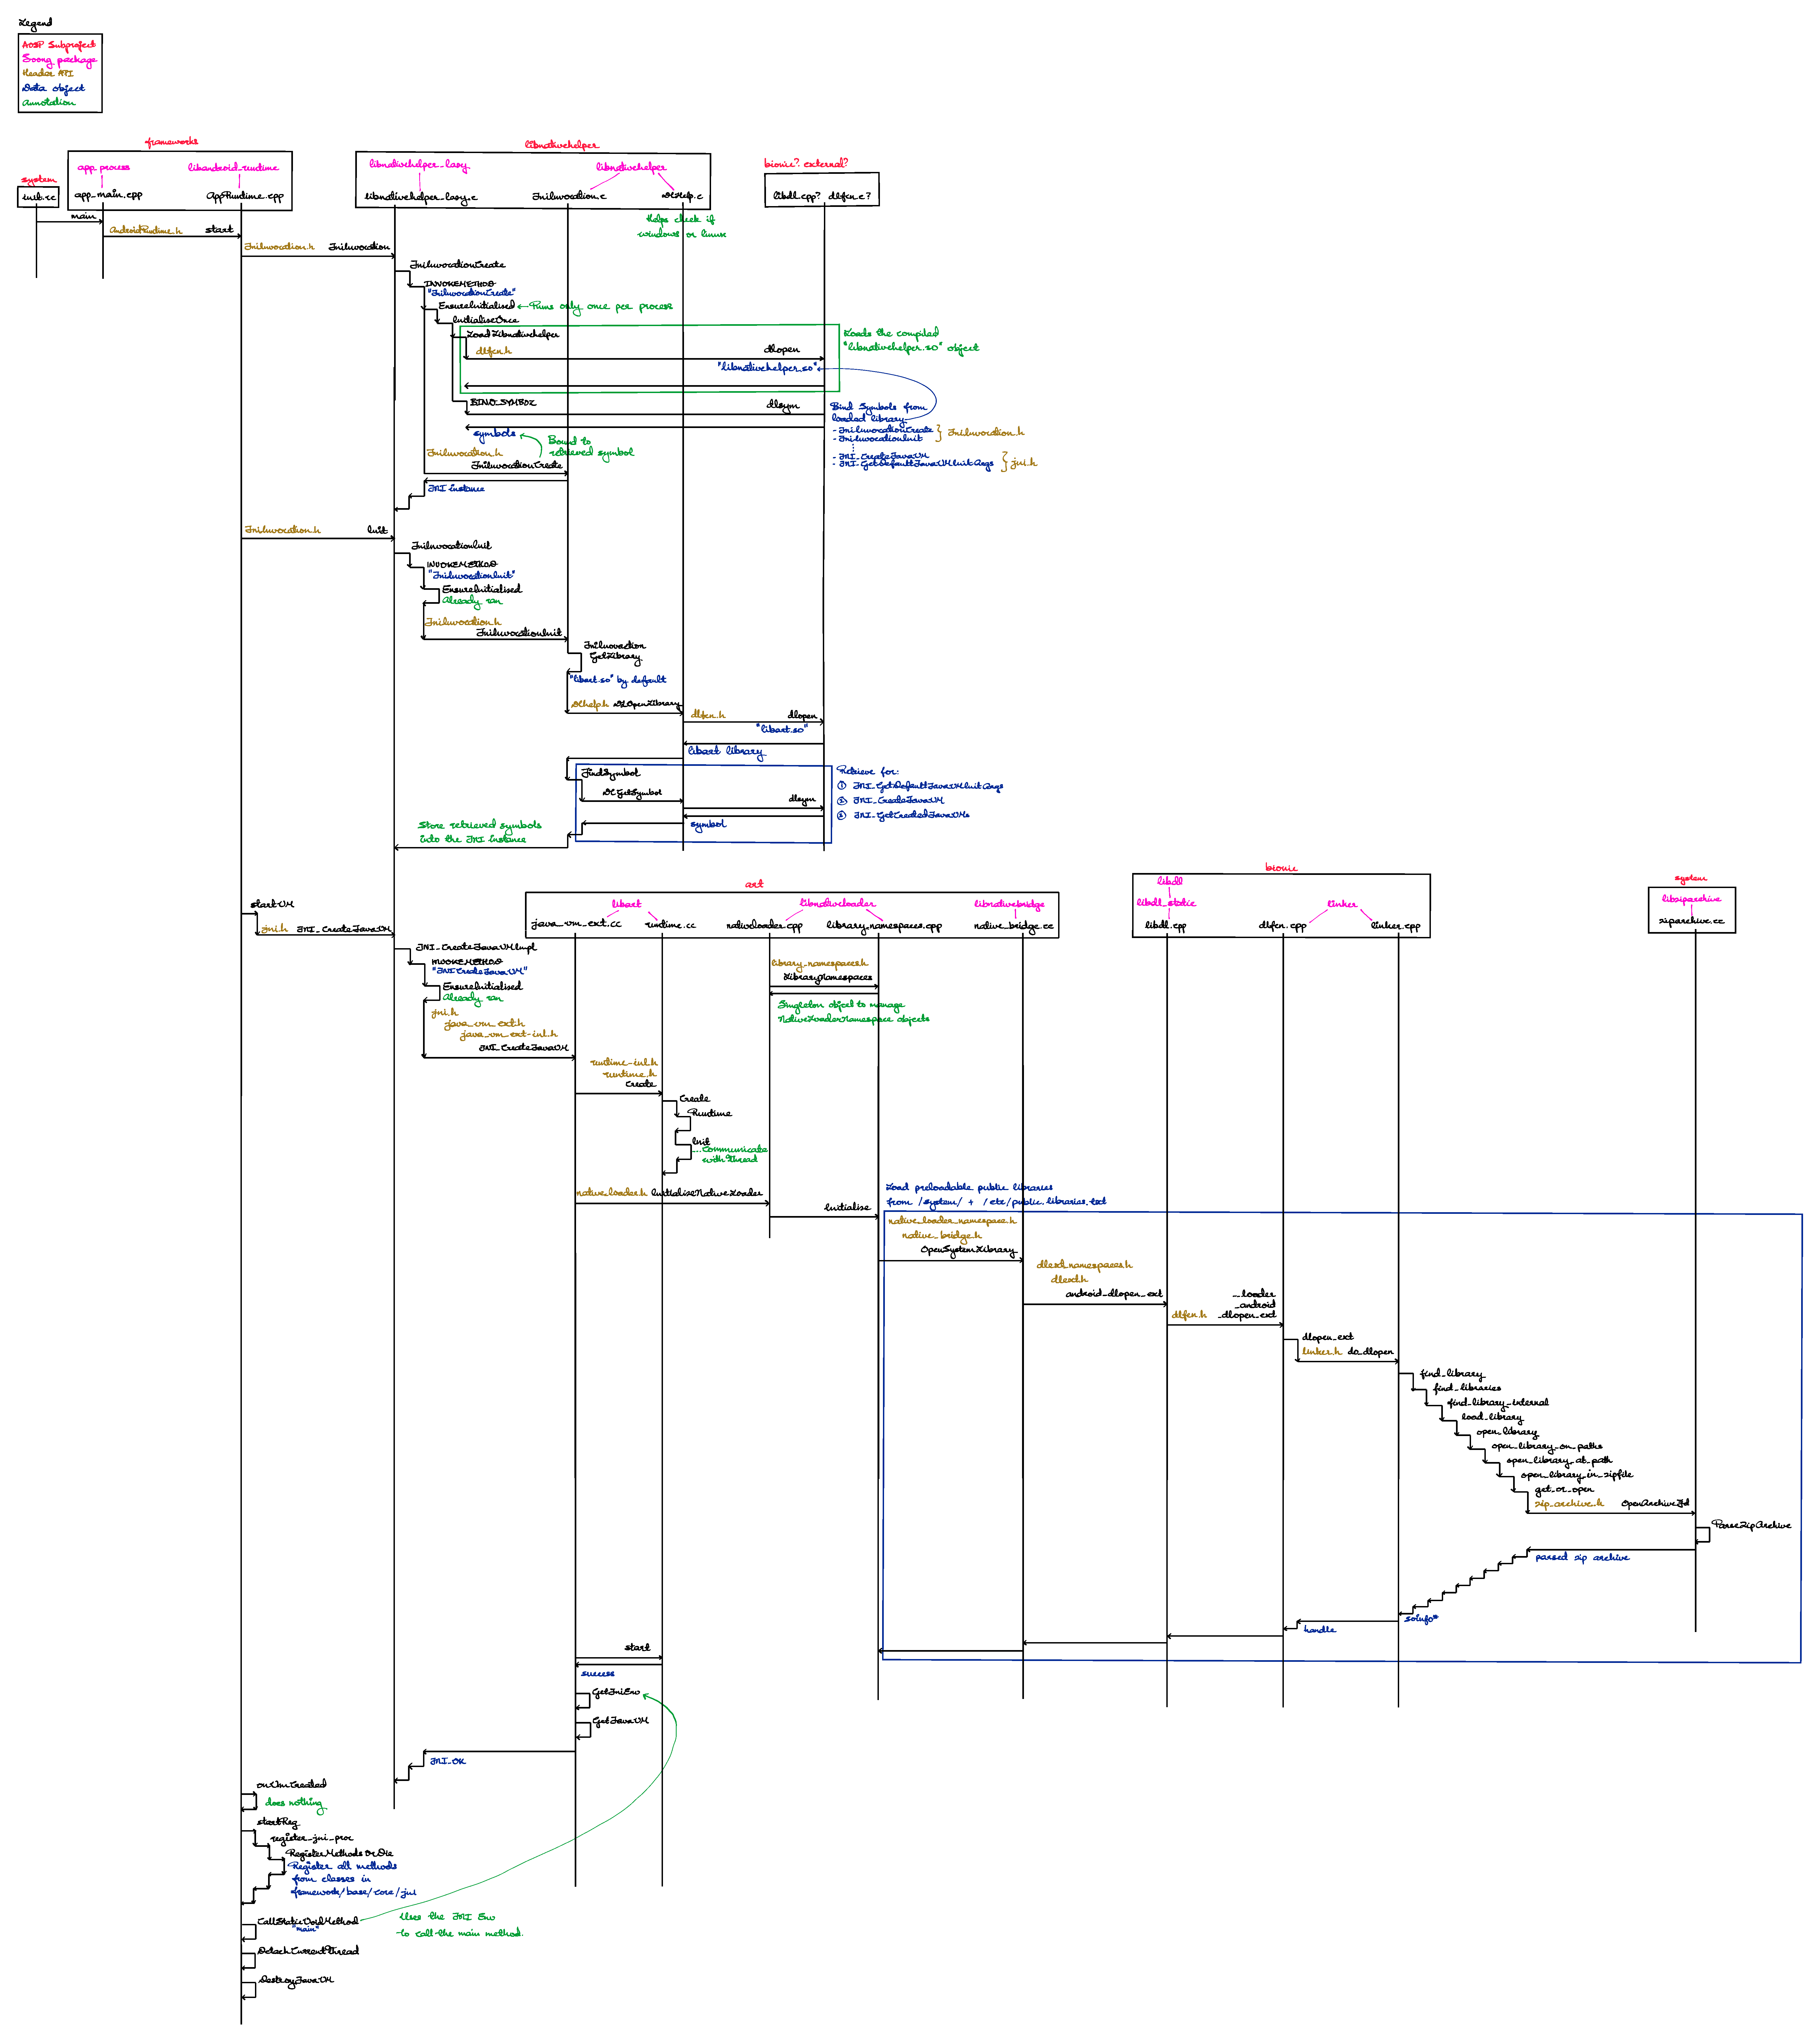
\includepdf[pages=-, scale=.95,pagecommand={}]{entries/2024/01/01/art.pdf}

% \begin{itemize}
% \item \textbf{Domain.} The context of the process that is acting upon something.
% \item \textbf{Type.} The context of the resource on which the process is acting.
% \item \textbf{Class.} The object class of the resource (e.g. \textit{file} or \textit{socket}).
% \item \textbf{Permissions.} The permissions that are allowed given the \textit{domain}, \textit{type} and \textit{class}.
% \end{itemize}

% SELinux rule syntax:


% \subsubsection{Decoding Permission Denial Message}

% Message:
% \begin{lstlisting}
% type=AVC msg=audit(1363289005.532:184): avc:  denied  { read } for  pid=29199 comm="Trace" 
% name="online" dev="sysfs" ino=30 scontext=staff_u:staff_r:googletalk_plugin_t 
% tcontext=system_u:object_r:sysfs_t tclass=file
% \end{lstlisting}

% \begin{longtable}{p{.15\linewidth}p{.15\linewidth}p{.65\linewidth}} 
% \toprule
% Log part & Name & Description \\
% \midrule
% \endhead

% \texttt{type=AVC}
% &Log type
% &Only in the \texttt{audit.log} file; it informs the user what kind of audit log type this is. 
% \\

% \midrule
% \caption{Permission Denied Syntax} 
% \label{tab:permissiondeniedsyntax}
% \end{longtable}


% \subsubsection{SELinux Architecture}

% SELinux consists of four main components: object managers (OM), access vector cache (AVC), security server, and security policy as show below:
% \begin{figure}[H]
%     \centering
%     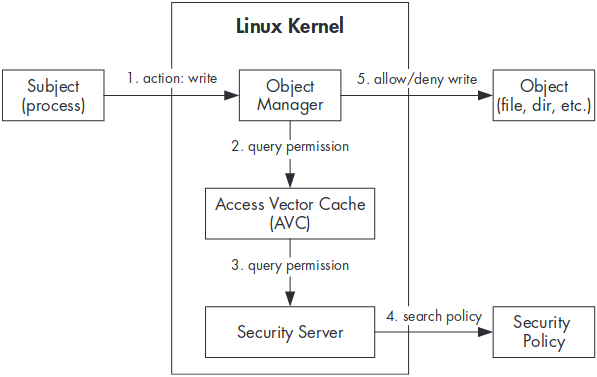
\includegraphics[width=.85\linewidth]{entries/2023/12/10/selinux.png}
%     \caption{SELinux Components}
%     \label{fig:selinux}
% \end{figure}
